\section{Our Approach}
\label{Sec:approach}
\vspace{-3pt}
Our regression testing approach is based on \emph{dynamic analysis} of \javascript code to infer invariants from a given web application. 
We use the thus obtained invariants as \emph{runtime assertions} in the \javascript code to automatically uncover regression errors that can be introduced after 
changes have been made to the web application in a subsequent reversion. Our approach is largely based on two assumptions (1) the current version of the web application, 
from which invariants are being generated, is bug-free (2) the inferred invariants capture program specifications that are unlikely to change frequently in the following revisions (we revisit these two assumptions in \secref{discussion}).
Our regression testing technique is composed of the following four main steps: (1) JavaScript tracing, (2) Invariant generation, (3) Filtering unstable assertions, and (4) Regression testing through assertions. In the following subsections, we will describe each step in details.


%\begin{enumerate}
%\item \textbf{JavaScript Tracing:} keeps track of and logs value changes during program execution;
%\item {\bf Invariant Generation:} infers program expressions that remain unchanged during multiple executions;
%\item {\bf Filtering Unstable Invariant Assertions:} removes reported false positives, i.e., any falsely detected invariant;
%\item {\bf Regression Testing through Invariant Assertions:} injects the generated invariants into the web application's code as assertions for detecting faults on a modified version of the web application;
%\end{enumerate}
%
%Our technique is concerned with the client-side code (e.g., \javascript, DOM) and
%is orthogonal to server-side technology.

\begin{figure}[t]
\centering
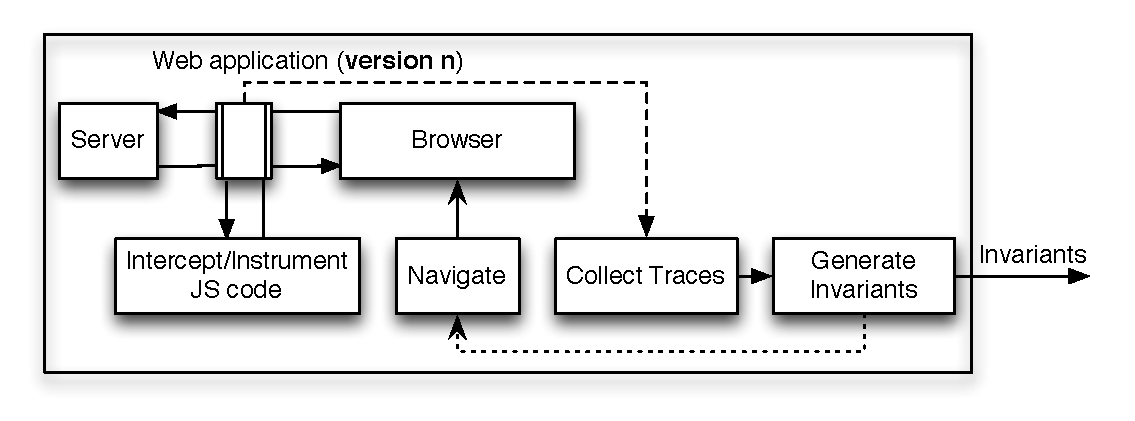
\includegraphics[width=0.9\hsize]{fig/approach-view}
\mycaption{Overview of the \javascript tracing and invariant generation steps (web application version \emph{n}).}
\label{Fig:invariantDetectionDiagram}
%\vspace{-0.3in}
\end{figure}


\subsection{\javascript Tracing}
In order to infer useful program invariants, we need to collect execution traces of the \javascript code. The idea is to log as much program variable value changes at runtime as possible.  \figref{invariantDetectionDiagram} depicts a block diagram of the tracing step. Our approach automatically generates trace data in three subsequent steps: 
(i) \javascript interception and instrumentation, (ii) navigation, and (iii) trace collection. In the following, we explain each step in details. 
%In our approach, we run the application using automated
% crawling technique \cite{?} with several different configurations. Each crawling configuration results in a new set of trace data.

\head{\javascript Interception and Instrumentation.} The approach we have chosen for logging variables is on-the-fly \javascript source code transformation to add instrumentation code.
We intercept all the \javascript code of a given web application, both in \javascript files and HTML pages, by setting up a proxy \cite{bezemer:esec09} between the server and the browser. We first parse the intercepted source code into an Abstract Syntax Tree (AST). 
We then traverse the AST in search of \emph{program variables} as well as \emph{DOM modifications} as described below.
% Once the code is instrumented, we
% serialize the AST back to the corresponding source code file and pass it to the browser.

{\bf Tracing Program Variables.} Our first interest is the range of values of \javascript program variables. We probe function entry and function exit points, by identifying function definitions in the AST and injecting statements at the start, end, and before every \code{return} statement. We instrument the code to monitor value changes of \emph{global variables}, \emph{function arguments}, and \emph{local variables}. 
Per program point, we yield information on \emph{script name}, \emph{function name}, and \emph{line number}, used for debugging purposes. Going back to our running example (\figref{motivating_example}), our technique adds instrumentation code to trace \code{width}, \code{height}, \code{h}, and \code{w}. For each variable, we collect information on \emph{name}, \emph{runtime type}, and \emph{actual values}. The runtime type is stored because \javascript is a loosely typed language, i.e., the types of variables cannot be determined syntactically, thus we log the variable types at runtime.

{\bf Tracing DOM Modifications.} In modern web applications, \javascript code
frequently interacts with the DOM to update the client-side user interface state. Our recent study \cite{ocariza:icst12} of four bug-tracking systems indicated that DOM-related errors form 80\% of all reported \javascript errors. Therefore,  we include in our execution trace how DOM elements and their attributes are modified by \javascript at runtime. 
For instance, by tracing how the CSS property of the `end' DOM element in \figref{motivating_example} is changed during various execution runs, we can infer the range of values for the \code{height} attribute. 

Based on our observations, \javascript DOM modifications usually follow a certain pattern. Once the pattern is reverse engineered, we can add proper instrumentation code around the pattern to trace the changes.
In the patterns that we observed, first a \javascript API is used to find the desired DOM element. Next, a function is called on the returned object responsible for the actual modification of the DOM-tree. After recognizing a pattern in the parsed AST, we add instrumentation code that records the value of the
DOM attribute before and after the actual modification. Hence, we are able to trace DOM modifications that happen programmatically through \javascript.

\head{Navigation.}
Once the AST is instrumented, we serialize it back to the corresponding \javascript source code file and pass it to the browser.
Next, we navigate the application in the browser to produce an execution trace. The application can be navigated in different ways including (1) manual clicking (2) test case execution (3) or using a web crawler. To automate the approach, our technique is based on automated dynamic crawling \cite{mesbah:tweb11}. The execution needs to run as much of the \javascript code as possible
and execute it in various ways. This can be achieved through visiting as many DOM state changes 
as possible as well as providing different values for function arguments.


\head{Trace Collection.} 
As the web application is navigated, the instrumented \javascript code produces trace data, which needs to be collected for further analysis. Keeping the trace data in the browser's memory during the program execution can make the browser slow when a large amount of trace data is being produced. On the other hand, sending data items to the proxy as soon as the item is generated, can 
put a heavy load on the proxy, due to the frequency of HTTP requests.
In order to tackle the aforementioned challenges, we buffer a certain amount of trace data in the 
memory in an array, post the data as an HTTP request to a proxy server when the buffer's size reaches a predefined threshold, and immediately clear the buffer in the browser's memory afterwards. Since the data arrives at the server in a synchronized manner, we concatenate the tracing data into a single trace file on the server side, which is then seeded into the next step (See \figref{invariantDetectionDiagram}).

%\figref{example_var_instrumentation} shows the automatically instrumented \javascript code for program local variables as well as function arguments.
%Similar to DOM modifications, we trace variables and function arguments through calling {\bf save} function. 
%In order to trace value changes of local variables, we instrument the \javascript code at exit point of the function. 
%However, to keep track of function arguments as well as global variables, we instrument the code at both entry and exit point of the function.  
%As shown in \figref{invariantDetectionDiagram}, we cycle through invariant
%detection phase until the size of retrieved invariant file remains unchanged. This implies that
%all possible invariants have been detected.

%\figref{invariantDetectionDiagram} and \figref{testingDiagram} 
%depict block diagram view of three main steps of our approach. The number in each box represents
% %sequence of the corresponding function. In the following, we describe each step in details.

\subsection{Invariant Generation}
The assertion generation phase is involved with analyzing the collected execution traces to extract invariants.   Substantial amount of research has been carried out on detecting dynamic program invariants \cite{agitator:issta06,Csallner08dysy,ernst2007daikon,Hangal02trackingdown}. Our approach is based on Daikon \cite{ernst2007daikon} to infer likely invariants. %, which uses a brute-force method: for all variables, consider all possible invariants to be true, iterate over the list of found values, and remove any invariant item that fails with any of these values.
% 
As indicated with the dotted line in \figref{invariantDetectionDiagram}, we cycle through the navigation and invariant generation phases until the size of generated invariant file remains unchanged, which is an indication that all possible invariants have been detected.
%In order to find useful invariants, we need to
%collect extensive execution traces. The execution 
%needs to run as much of the \javascript code, as possible
%and execute it in various ways. This can be achieved through visiting as many DOM state changes 
%as possible as well as providing different values for function arguments. However, manually producing
%extensive execution traces would be too expensive. It is possible to use a test suite that uses
%browser controlling libraries such as Selenium \cite{?}. In case that test suites are non-existent or 
%not able to generate enough trace data, automated crawling techniques \cite{?} can
%be used to produce execution traces. In our approach, we run the application using automated
%crawling tool with several different configurations. Each crawling configuration results in a 
%new set of invariants. As shown in \figref{invariantDetectionDiagram}, we cycle through invariant
%detection phase until the size of retrieved invariant file remains unchanged. This implies that
%all possible invariants have been detected.

\begin{figure}[t]
\centering
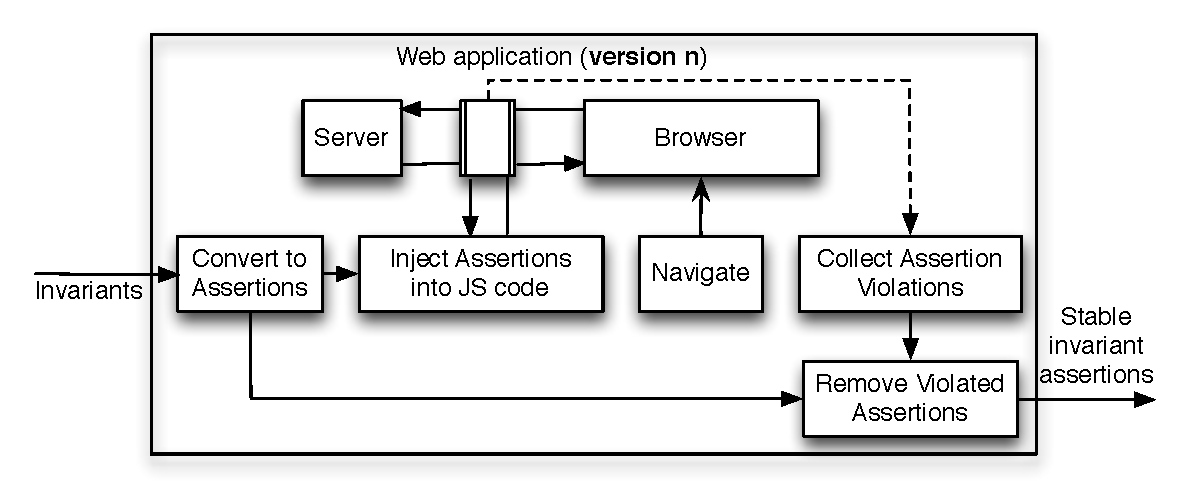
\includegraphics[width=0.9\hsize]{fig/filter-test}
\mycaption{Overview of the filtering step to remove unstable invariant assertions, for web application version \emph{n}.}
\label{Fig:filtering}
%\vspace{-0.3in}
\end{figure}


\subsection{Filtering Unstable Invariant Assertions}
\label{Sec:filtering}
The next step is to make sure that the generated invariants are truly invariants. 
An invariant assertion is called unstable when it is falsely reported as a violated assertion. Such assertions result in producing a number of false positive errors 
during the testing phase. 
To check the stability of the inferred invariants, we use them in the same version of the web application as assertions. Theoretically, no assertion violations should be reported because the web application has not changed. Hence, any assertion violation reported as such is a false positive and should be eliminated. Our filtering process, shown in \figref{filtering}, consists of the following four processes:

\begin{itemize}
\item Converting the inferred invariants into checkable assertions;
\item Injecting the invariant assertions into the same version of the web application;
\item Navigating the web application;
\item Collecting assertion violations and removing them;
\end{itemize}
% In order to test the stability of inferred invariants, we automatically convert them into checkable assertions.
% Derived Assertions are instrumented in the original application code and will be checked at run time.
% We then atomatically detect violated assertions in the output report and remove corresponding invariants.
% The new obtained set of invariants are stable and will be used in our regression testing phase.



From each of the inferred invariants, we generate an assertion in \javascript format. We use on-the-fly transformation to inject the assertions directly into the source code of the same version of the web application. Since we have all the information about the program points and the location 
of the assertions, we can inject the assertions at the correct location in the \javascript source code through the proxy, while the code is being  
 sent to the client by the server. This way the assertions can run as part of the client-side code and gain access to the values of all program variables needed at runtime. Once the assertions are injected, we execute the web application in the browser and log the output. Next we collect and remove any violated assertions. The output of this step is a set of \emph{stable} invariant assertions, used for automated regression testing in the next step.

\subsection{Regression Testing through Assertions}
Once a set of stable invariant assertions are derived from version \code{n} of a web application, they can be used for automatic regression testing a subsequent version (\code{n+1}) of the web application. The regression testing phase is depicted in \figref{testingDiagram}.


%\begin{itemize}
%\item Injecting the stable invariant assertions into the subsequent version of the web applicatoin;
%\item Navigating the web application;
%\item Logging the output of the assertions when they fail, and reporting the test results.
%\end{itemize}
 


\begin{figure}[t]
\centering
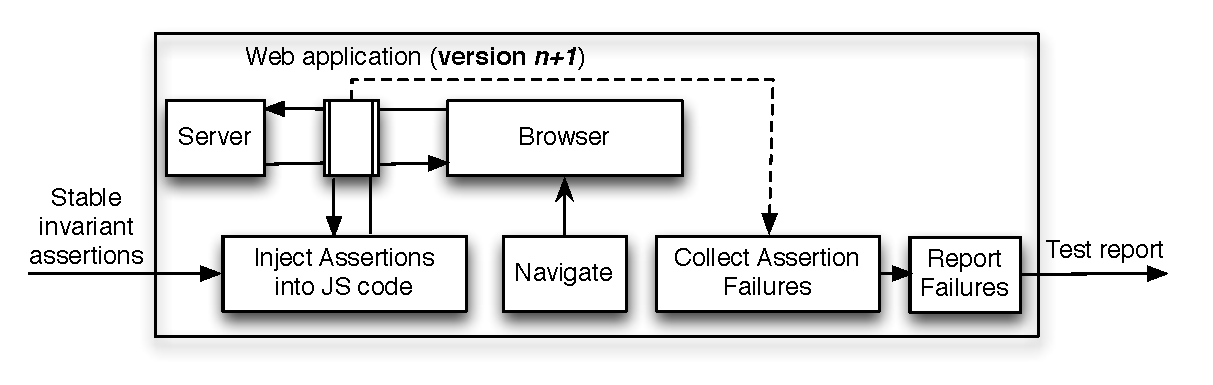
\includegraphics[width=0.9\hsize]{fig/regression-testing}
\mycaption{Overview of the \javascript regression testing step through invariant assertions, for web application version \emph{n+1}.}
\label{Fig:testingDiagram}
\end{figure}

We inject the inferred stable assertions to the \javascript source code of the modified web application, in a similar fashion to the filtering step in \secref{filtering}. Once the assertions are injected, the new version of the web application is ready for regression testing. Any failed assertion during the testing phase generates an entry in the test report, which is presented to the tester at the end of the testing step.
The generated test report provides precise information on the failed assertion, the file name,  the line number, and the function name of the assertion.

\begin{figure}[h]
%\medskip

\begin{mdframed}
\begin{lstlisting}[frame=none]
	function setDim(height, width) {
		[\textbf{assert((width < height), `example.js:setDim:ENTER:POINT1');}] 			
		var h = 4*height, w = 2*width;		
		...
		[\textbf{assert((width < height), `example.js:setDim:EXIT:POINT1');}]
		[\textbf{assert((w < h), `example.js:setDim:EXIT:POINT1');}]
		return{h:h, w:w};
	}

	function play(){
		$(#end).css("height", setDim($('body').width(), $('body').height()).h + 'px');
		[\textbf{assert(isIn(\$(`\#end').css(`height'), \{100, 200, 	300\}),`example.js:play:POINT3');}]
		...
	}
\end{lstlisting}
\end{mdframed}
\vspace{.2in}
\mycaption{Invariant assertion code for \javascript function parameters, local variables and DOM modifications. Injected assertions are shown in bold.}
\label{Fig:example_assertion}
\end{figure}


\figref{example_assertion} shows the automatically injected invariant assertions for our running example of
\figref{motivating_example}. Note that we do not show all the assertions as they clutter the figure. Each \code{assert} call has the invariant as the first parameter and the corresponding debugging information in the second parameter, which includes information about script name, function name, and line number.
In this example, the inferred invariants yield information about the inequality relation between function arguments, \code {width} and \code {height}, as well as local variables, \code{w} and \code{h}. 
The assertions in lines 2 and 5-6 check the corresponding inequalities, at entry and exit points of the \code{setDim} function at runtime. 
% Similarly, assertion for testing local variables, \code {w} and \code {h}, is called before function returns. 
%In addition to the function arguments, the example also shows the assertions that check the \code{height} attribute of the DOM element, before and after the \javascript DOM modification. 
%The assertion that comes before the DOM manipulation checks the \code {height} value to be equal to 40, while the succeeding assertion checks the \code {height} to be either 200 or 400. Any other values would violate the assertions.
The example also shows the assertion that checks the \code{height} attribute of the DOM element, after the \javascript DOM modification in the \code{play} function. 
The assertion that comes after the DOM manipulation (Line 12) checks the \code {height} value by calling the auxiliary \code{isIn} function. \code{isIn} checks the  value of \code{height}
to be in the given range, i.e., either 100, 200, or 300. Any values out of the specified range would violate the assertion.


 




